\section{Dữ liệu 2: Hồi quy thành phần chính}

\subsection*{Giới thiệu bộ dữ liệu}
Hiện nay, Xe đạp cho thuê được giới thiệu ở nhiều thành phố để nâng cao sự thoải~mái khi di chuyển. Điều cần quan tâm khi cho thuê xe đạp là xe đạp phải luôn sẵn sàng và tiếp cận được người dùng vào đúng thời điểm, giúp giảm bớt thời gian chờ. Do đó, việc đảm bảo một nguồn cung cấp xe đạp cho thuê ổn định cho thành phố trở thành mối~quan~tâm lớn. Phần quan trọng là cần dự đoán được số lượng xe đạp cần thiết tại mỗi~giờ, để có được nguồn cung cấp xe đạp cho thuê ổn định.

\textbf{Bộ dữ liệu:} Nhu cầu thuê xe đạp ở Seoul\footnote{\url{https://archive.ics.uci.edu/ml/datasets/Seoul+Bike+Sharing+Demand}} (\textbf{Seoul Bike Sharing Demand Dataset}) ghi lại các thông tin về thời tiết, số lượng xe đạp được thuê mỗi giờ theo từng ngày, từ 01/12/2017 đến 31/11/2018. Bộ dữ liệu có 8760 quan trắc, gồm 14 biến:
\begin{enumerate}
	\item \texttt{Date} - Ngày ghi lại số lượng xe đạp cho thuê
	\item \texttt{Rented Bike count} - Số lượng xe đạp được thuê được ghi lại theo mỗi giờ
	\item \texttt{Hour} - Giờ trong ngày
	\item \texttt{Temperature} - Nhiệt độ ($^o C$)
	\item \texttt{Humidity} - Độ ẩm (\%)
	\item \texttt{Windspeed} - Tốc độ gió ($m/s$)
	\item \texttt{Visibility} - Tầm nhìn xa ($10m$)
	\item \texttt{Dew point temperature} - Nhiệt độ điểm sương ($^o C$)
	\item \texttt{Solar radiation} - Bức xạ mặt trời ($Mj/m^2$)
	\item \texttt{Rainfall} - Lượng mưa ($mm$)
	\item \texttt{Snowfall} - Lượng tuyết rơi ($cm$)
	\item \texttt{Seasons} - Mùa (Winter, Spring, Summer, Autumn)
	\item \texttt{Holiday} - Ngày lễ (Holiday/No holiday)
	\item \texttt{Functional Day} - Ngày làm việc (Yes nếu là ngày làm việc, No nếu ngược lại)
\end{enumerate}

Một vài quan trắc đầu tiên trong bộ dữ liệu được thể hiện trong hình \ref{A2_head}

\begin{figure}[H]
	\centering
	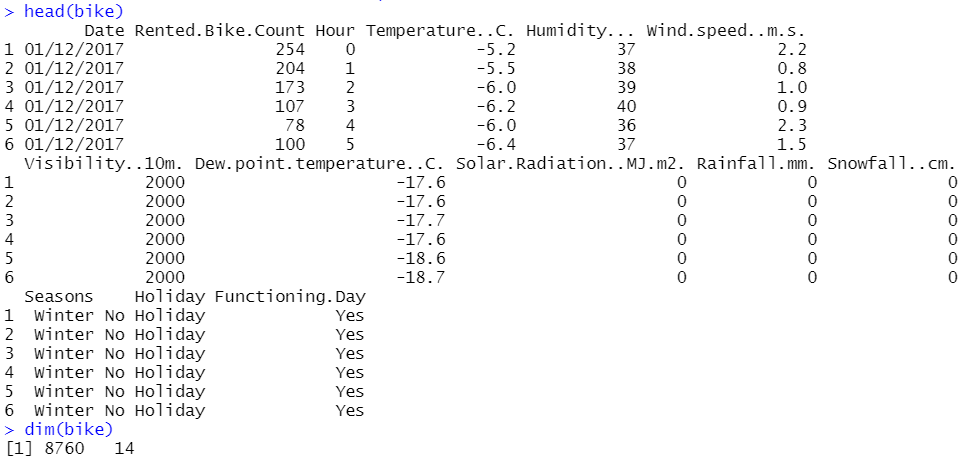
\includegraphics[width=0.7\linewidth]{../Photo Of Result/A2_head}
	\caption{Một vài quan trắc đầu tiên và số chiều của bộ dữ liệu}
	\label{A2_head}
\end{figure}

Vì mục đích bài toán là dự đoán số lượng xe đạp theo mỗi giờ, do đó nhóm em loại bỏ biến \texttt{Date}. Bên cạnh đó, các biến định tính cũng được biến đổi thành các biến dummy, cụ thể: \texttt{Hour} được phân rã thành 24 biến, \texttt{Seasons} được phân rã thành 4 biến, \texttt{Holiday} mang giá trị 1 nếu là Holiday và 0 nếu ngược lại, \texttt{Functional Day} mang giá~trị 1 nếu là Yes và 0 nếu ngược lại. Lúc này bộ dữ liệu gồm 39 biến.

\begin{figure}[H]
	\centering
	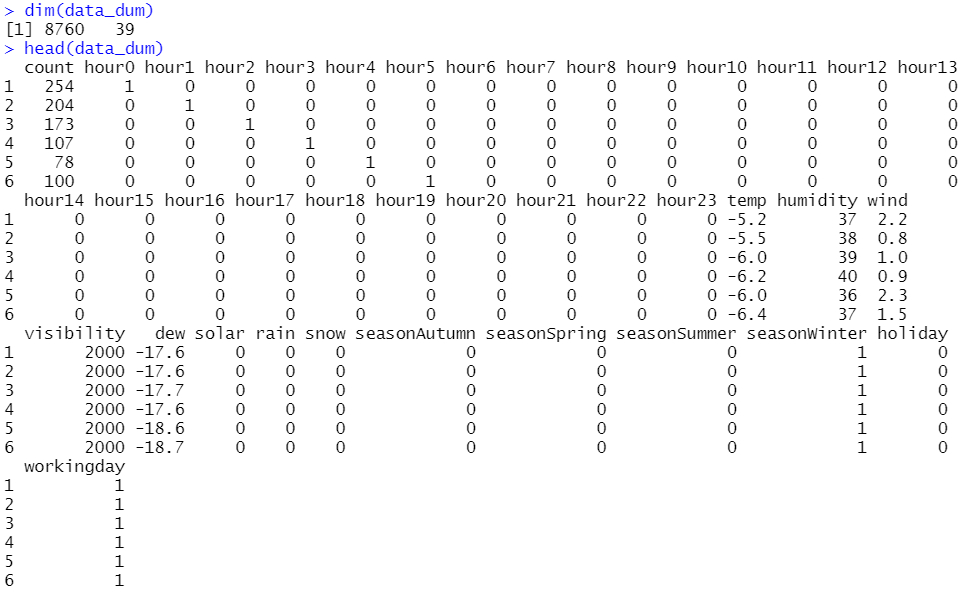
\includegraphics[width=0.7\linewidth]{../Photo Of Result/A2_dummy}
	\caption{Dữ liệu sau khi loại bỏ \texttt{Date} và tạo các biến giả}
	\label{A2_head2}
\end{figure}

\subsection*{Phân tích và chọn mô hình}

\begin{figure}[H]
	\centering
	{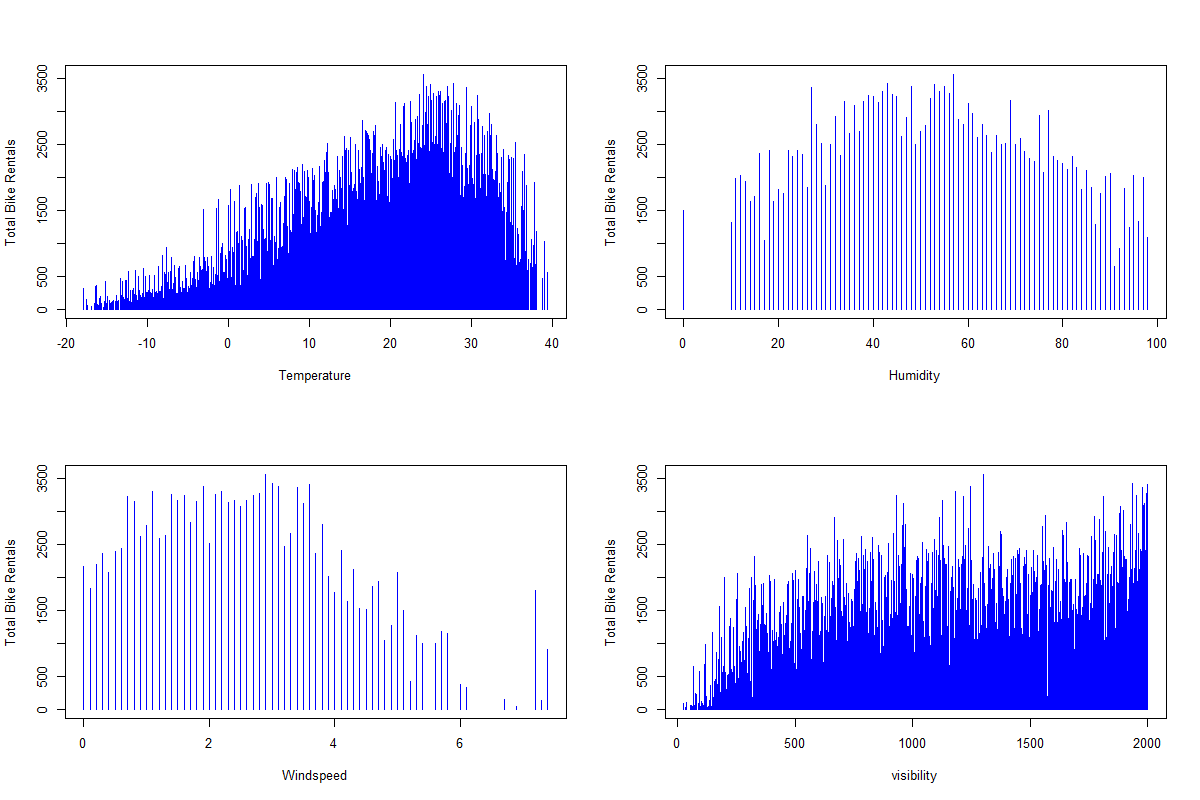
\includegraphics[width=.8\linewidth]{../Photo Of Result/A2_plotvar1}}\\
	{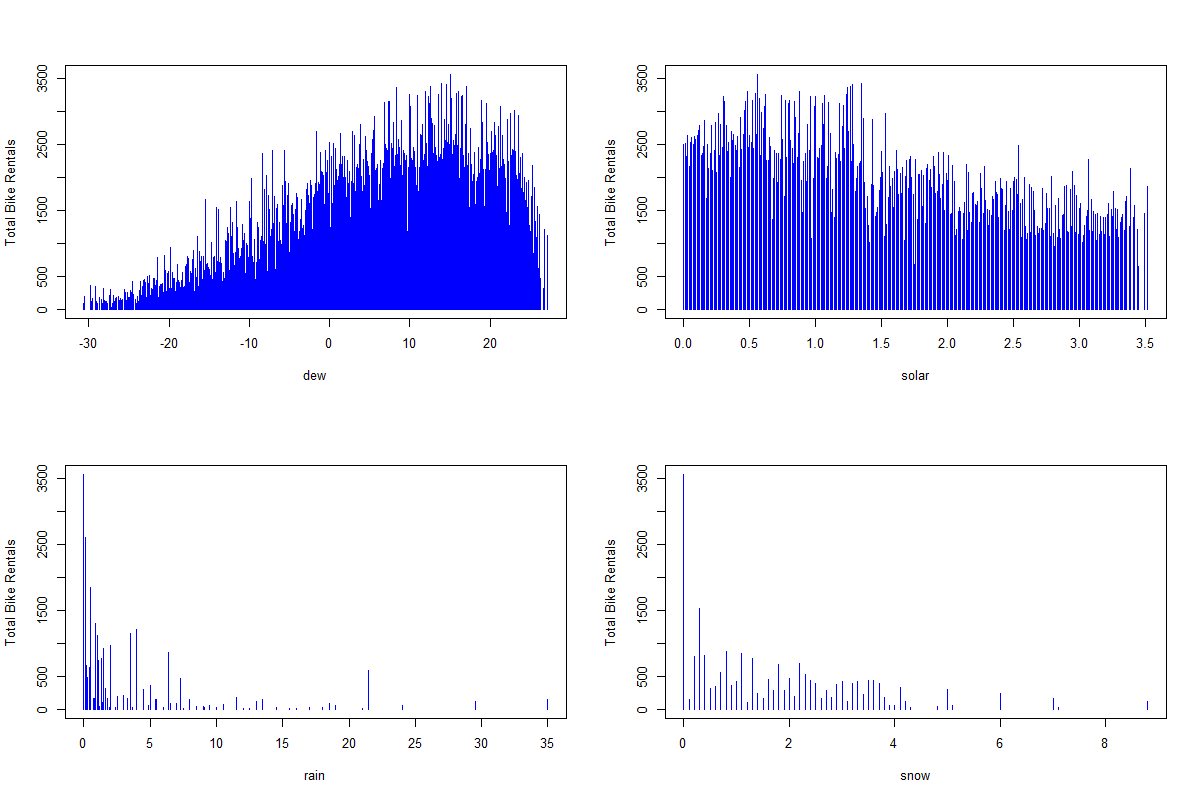
\includegraphics[width=.8\linewidth]{../Photo Of Result/A2_plotvar2}}
	\caption{Quan sát phân bố của từng biến với \texttt{Count}}
	\label{A2_visual1}
\end{figure}

Các kết quả từ hình \ref{A2_visual1} cho thấy xe đạp được thuê nhiều khi nhiệt độ (\texttt{Temp}) và nhiệt độ điểm sương (\texttt{Dew}) 

\begin{figure}[H]
	\centering
	{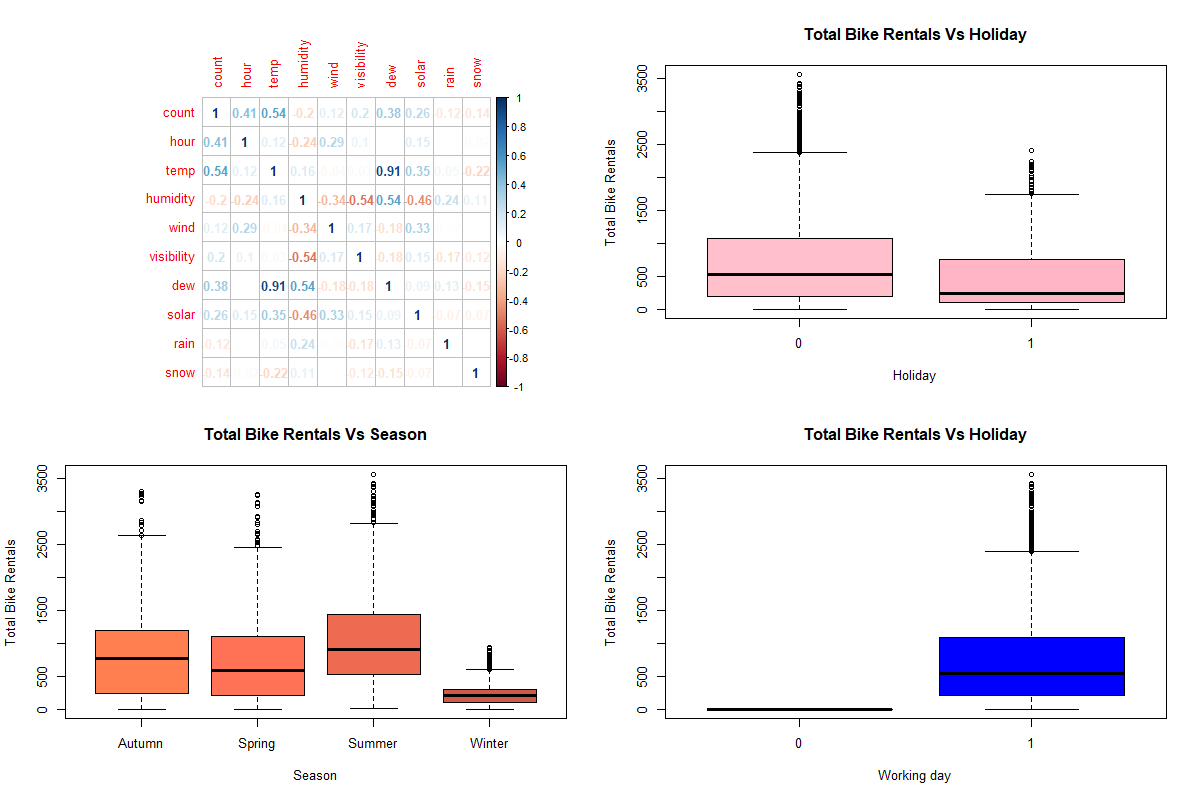
\includegraphics[width=\linewidth]{../Photo Of Result/A2_corr}}	
	\caption{Quan sát ma trận hiệp phương sai và các biến định tính}
	\label{A2_visual2}
\end{figure}

%Từ những quan sát về kiểu dữ liệu và mối tương quan giữa các biến độc lập với nhau cũng như giữa các biến độc lập và biến phụ thuộc ta thấy: Mô hình nhóm đi phân tích gồm 8 biến độc lập liên tục, 4 biến độc lập kiểu phân loại. Một trong số chúng có mối tương quan mạnh mẽ với nhau như biến \texttt{Dew point temperature} và hai biến \texttt{Temperature}, \texttt{Humidity}. mặt khác,  Để giải quyết vấn đề của bộ dữ liệu có số biến lớn và có mối tương quan mạnh giữa các biến độc lập với nhau nhóm sẽ dùng phương pháp tiếp cận giảm chiều dữ liệu (PCA) để biến đổi dữ liệu về không gian có số chiều nhỏ hơn mà vẫn giữ được nhiều thông tin nhất có thể của bộ dữ liệu.

\begin{figure}[H]
	\centering
	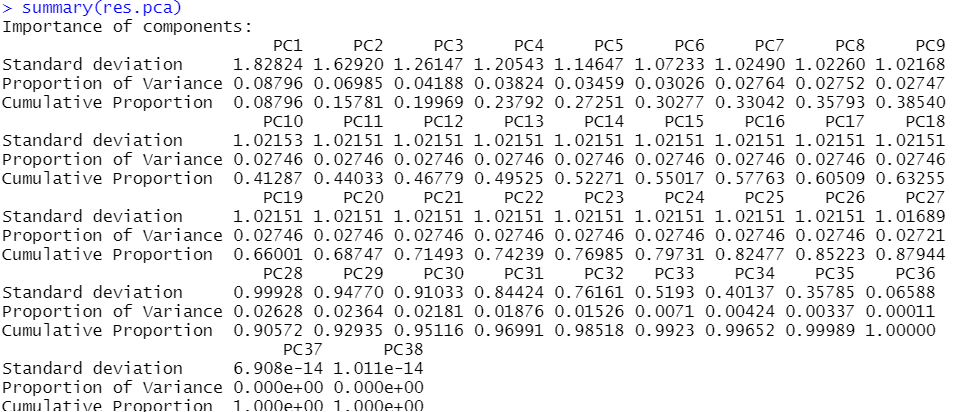
\includegraphics[width=0.9\linewidth]{../Photo Of Result/A2_PCproportion.PNG}
	\caption{Kết quả PCA}
	\label{A2_PCAmod1}
\end{figure}

\begin{figure}[H]
	\centering
	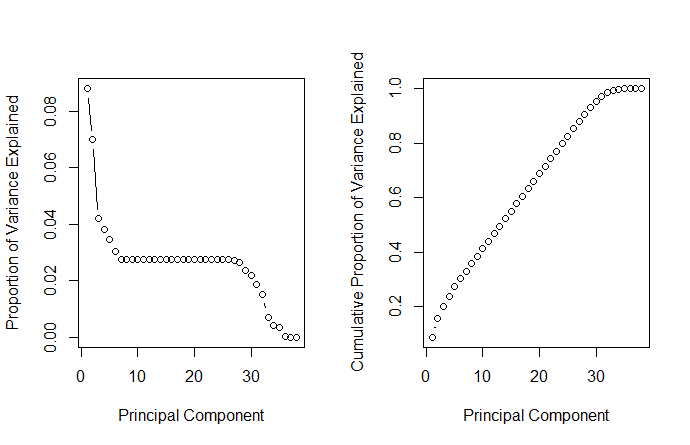
\includegraphics[width=0.9\linewidth]{../Photo Of Result/A2_pca_plotvar.png}
	\caption{Thành phần chính}
	\label{A2_Var}
\end{figure}


%Dựa vào kết quả PCA được xuất ra từ phần mềm R ta thấy 26 thành phần chính đầu tiên giải thích được khoảng 85 $\%$ tập dữ liệu ban đầu. Thực hiện hồi quy tuyến tính trên những thành phần chính này thu được kết quả hồi quy như hình \ref{A2_model26PCA}. \\


%Mô hình giải thích được khoảng 50 $\%$ ($R^{2}$) cho sự thay đổi số lượng thuê xe đạp tại Seoul. Tuy nhiên trong mô hình hồi quy vẫn chưa những biến \texttt{PC7}, \texttt{PC13}, và \texttt{PC14} không có ý nghĩa thống kê do $\rho_{value} \ge \alpha$ hình \ref{A2_model26PCA}.

%Tiến hành loại bỏ những biến này ra và thực hiện hồi quy tuyến tính trên tập biến mới hình \ref{A2_summaryPCA2}. $R^{2} \approx 49.5 \% $ không thay đổi nhiều so với mô hình trước đó. Tuy nhiên trong mô hình mới này tất cả những biến độc lập đều có ý nghĩa thống kê do $\rho_{value} \ge \alpha$.

\begin{figure}[H]
	\centering
	\subfloat[Hồi quy với 26 thành phần chính đầu tiên]
	{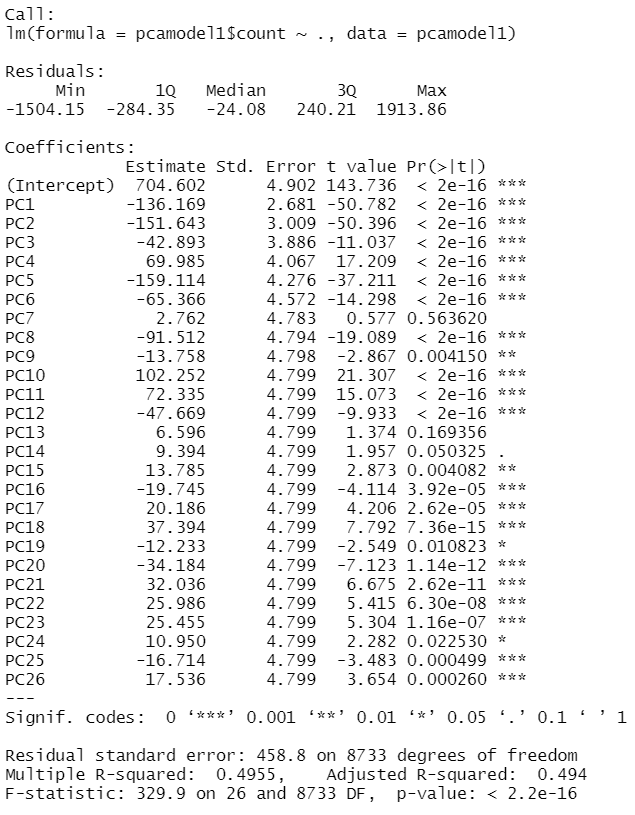
\includegraphics[width=0.5\linewidth]{../Photo Of Result/A2_pca_mod1.PNG}} \hfill
	\subfloat[Hồi quy với 23 thành phần chính]
	{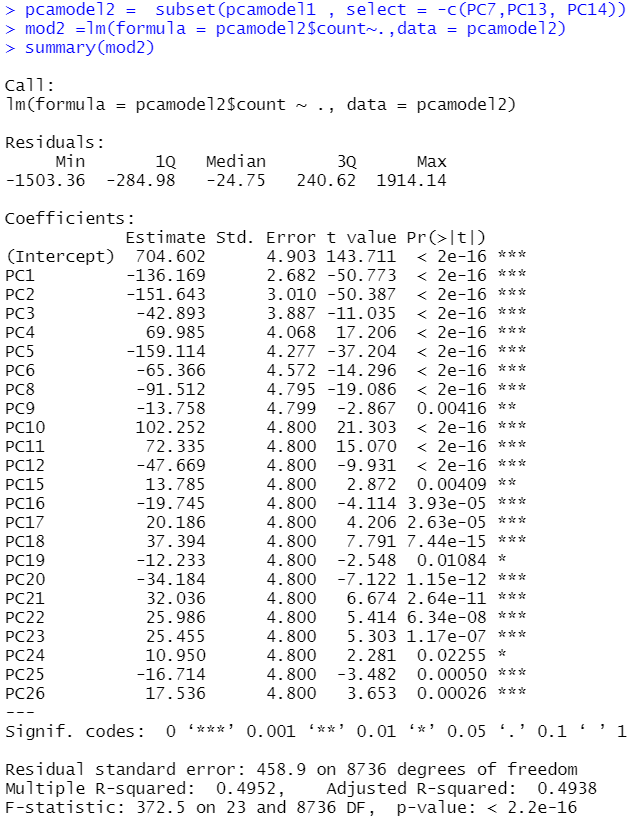
\includegraphics[width=0.5\linewidth]{../Photo Of Result/A2_pca_mod2.PNG}}
	\caption{Hồi quy thành phần chính}
	\label{A2_modPCA}
\end{figure}


\subsection*{Nhận xét và kết luận}